

%\newcommand*{\ACM}{}%

\ifdefined\ACM

%\documentclass[sigplan,screen]{acmart}
  \documentclass[manuscript,screen,review]{acmart}

\else
  \documentclass{article}
  \usepackage[utf8]{inputenc}
\usepackage[a4paper, total={6in, 9in}]{geometry}
\usepackage{braket}
\usepackage{xcolor}
\usepackage{amsmath}
\usepackage{amsfonts}
\usepackage{amsthm}
\usepackage{amssymb}
%\usepackage[ocgcolorlinks]{hyperref}
\usepackage{hyperref}
%\usepackage{hyperref,xcolor}
%\usepackage[ocgcolorlinks]{ocgx2}
\usepackage{cleveref}
\usepackage{graphicx}
\usepackage{svg}
\usepackage{float}
\usepackage{tikz}
\usetikzlibrary{patterns, shapes.arrows}
\usepackage{adjustbox}
%\usepackage{tikz-network}
\usepackage{tkz-graph}
\usepackage{tkz-berge}
\usepackage[linesnumbered]{algorithm2e}
\usepackage{multicol}
\usepackage[backend=biber,style=alphabetic,sorting=ynt]{biblatex}
%\usepackage{xcolor}
%\usepackage{tkz-berge}
%\usepackage{tkz-graph}
\usepackage{pgfplots}
\usepackage{sagetex}
\usepackage{setspace}
\usepackage{etoc}
%\usepackage{wrapfig}
\usepackage{pgfgantt}
\DeclareUnicodeCharacter{2212}{−}
\usepgfplotslibrary{groupplots,dateplot}
\pgfplotsset{compat=newest}

\newtheorem{theorem}{Theorem}
\newtheorem{definition}{Definition}
\newtheorem{example}{Example}
\newtheorem{claim}{Claim}
\newtheorem{fact}{Fact}
\newtheorem{remark}{Remark}
\newtheorem*{theorem*}{Theorem}
\newtheorem{lemma}{Lemma}
\crefname{lemma}{Lemma}{Lemmas}
\hypersetup{colorlinks=true}
% , allcolors=blue,allbordercolors=blue,pdfborderstyle={0 0 1}}
%\hypersetup{pdfborder={2 2 2}}
% pdfpagemode=FullScreen,
% backref 

\newtheorem{problem}{Problem}
\crefname{problem}{Problem}{Problems}

\DeclareMathOperator{\Ima}{Im}


  \addbibresource{./sample.bib} 

\fi

\begin{document}
\newcommand{\commentt}[1]{\textcolor{blue}{ \textbf{[COMMENT]} #1}}
\newcommand{\ctt}[1]{\commentt{#1}}
\newcommand{\prb}[1]{ \mathbf{Pr} \left[ #1 \right]}
\newcommand{\prbm}[2]{ \mathbf{Pr}_{ #2 }\left[ #1 \right]}
\newcommand{\prbc}[3]{ \mathbf{Pr}_{ #2 }\left[ #1 \right | #3]}
\newcommand{\prbcprb}[3]{ \prbc{#2}{#1}{#3} \cdot \prb{#3} } 
\newcommand{\expp}[1]{ \mathbf{E} \left[ {#1} \right]}
\newcommand{\onotation}[1]{\(\mathcal{O} \left( {#1}  \right) \)}
\newcommand{\ona}[1]{\onotation{#1}}
\newcommand{\PSI}{{\ket{\psi}}}
\newcommand{\xij} { X_{ij} } 
\DeclareMathOperator{\Ima}{Im}
%\newcommand{\LESn}{\ket{\psi_n}}
%\newcommand{\LESa}{\ket{\phi_n}}
%\newcommand{\LESs}{\frac{1}{\sqrt{n}}\sum_{i}{\ket{\left(0^{i}10^{n-i}\right)^{n}}}}
%\newcommand{\Hn}{\mathcal{H}_{n}}
%\newcommand{\Ep}{\frac{1}{\sqrt{2^n}}\sum^{2^n}_{x}{ \ket{xx}}}
%\newcommand{\HON}{\ket{\psi_{\text{honest}}}}
%\newcommand{\Lemma}{\paragraph{Lemma.}}
\newcommand{\Cpa}{[n, \rho n, \delta n]}
%\setlength{\columnsep}{0.6cm}
\newcommand{\Jvv}{ \bar{J_{v}} } 
\newcommand{\Cvv}{ \tilde{C_{v}} } 

\newcommand{\Gz}{ G_{z}^{\delta} } 
\newcommand{ \Tann } {  \mathcal{T}\left( G, C_0 \right) }
\newcommand{\ireducable}{ireducable \hyperref[ire]{[\ref{ire}]} }
\newcommand{\cutUU}{E(U_{-1} \bigcup U_{+1} ,U)} 
\newcommand{\wcutUU}{w\left( E(U_{-1} \bigcup U_{+1} ,U)  \right)}
\newcommand{\testgo}{  \mathcal{T}\left(J, q , C_{0}\right) } 

\newcommand{\duC}{\left( C_{A}^{\perp}\otimes C_{B}^{\perp} \right)^{\perp}}
\newcommand{\duduC}{\left( C_{A}\otimes C_{B}\right)^{\perp}}
  




\title{Magic States Distillation  Using $\Delta$-Toric (good qLDPC?). } 
\author{David Ponarovsky}
\maketitle

%\begin{abstract}
%  We studies the complexity of synthesis quantum states using PRS, our reasch continues the work by \cite{searchtodecision}, \cite{rosenthal2023efficient}, \cite{rosenthal2021interactive}, \cite{metger2023stateqip}, \cite{delavenne2023quantum}.
%\end{abstract}
%

Let $\ket{f}$ be a codeword in $C_{X}$, and let $X_{g}$ be the indicator that equals $1$ if $f$ has support on $X_{g}$, and $0$ otherwise. Observes that applying $T^{\otimes}$ on $\ket{f}$ yilds the state: 
\begin{equation*}
  \begin{split}
    T^{\otimes n}\ket{f} & =  T^{\otimes n}\ket{\sum_{g} X_{g}g } = \exp \Big( i\pi/4 \sum_{g} X_{g}|g|  -  2 \cdot i \pi/4 \sum_{g,h} X_{g}X_{h}|g\cdot h| \\
    & +  4 \cdot i\pi/4 \sum_{g,h} X_{g}X_{h}X_{l}|g\cdot h \cdot l| -   8  \cdot i\pi/4 \cdot \text{ integers } \Big) \ket{f} \\
    & = \exp \Big( i\pi/4 \sum_{g} X_{g}|g|  -  2 \cdot \pi/4 \sum_{g,h} X_{g}X_{h}|g\cdot h| +  4 \cdot i\pi/4 \sum_{g,h} X_{g}X_{h}X_{l}|g\cdot h \cdot l| \Big) \ket{f}
  \end{split}
\end{equation*}

Now assume that the code $C_{X}$ is the quantum Tanner code, denote by $G,A,B$ the group and the two generator sets that are used for constructing the square complex. In addition, let us assume the existence of $d \in G$ such that $d$ is non-identity and commutes with any element in $A \cup B$. Then, observe that multiplying by $d$ preserves adjacency on the complex. Namely, if $\{u,v\} \in E$ then also $\{du, dv\} \in E$. 

Consider $\ket{f}$ such that if $X_g$ is not zero, and $g$ is associated with a local codeword $c \in C_A \otimes C_B$ on vertex $v$, then the generator associated with the local codeword $c$ on vertex $d \cdot v$ also supports $f$, denoted by $g'$. Thus, the exponent above becomes:

\begin{equation*}
  \begin{split}
    & = \exp \Big( i\pi/4 \sum_{g} X_{g}|g|  -  2 \cdot \pi/4 \sum_{g,h \in G /a} X_{g}X_{h}|g\cdot h| + X_{g^{\prime}}X_{h^{\prime}}|g\cdot h |  \\
    & +  4 \cdot i\pi/4 \sum_{g,h \in G/a} X_{g}X_{h}X_{l}|g\cdot h \cdot l| + X_{g^{\prime}}X_{h^{\prime}}X_{l^{\prime}}|g\cdot h \cdot l| \Big) \ket{f} \\
    & = \exp \Big( i\pi/4 \sum_{g} X_{g}|g|  -  2 \cdot 2 \cdot \pi/4 \sum_{g,h \in G/a} X_{g}X_{h}|g\cdot h| +  2 \cdot 4 \cdot i\pi/4 \sum_{g,h \in G/a} X_{g}X_{h}X_{l}|g\cdot h \cdot l| \Big) \ket{f} \\
    & = \exp \Big( i\pi/4 \sum_{g} X_{g}|g|  -  i\pi \sum_{g,h \in G/a} X_{g}X_{h}|g\cdot h|  \Big) \ket{f} 
  \end{split}
\end{equation*}

\begin{figure}
  \centering
  \scalebox{0.1}{
    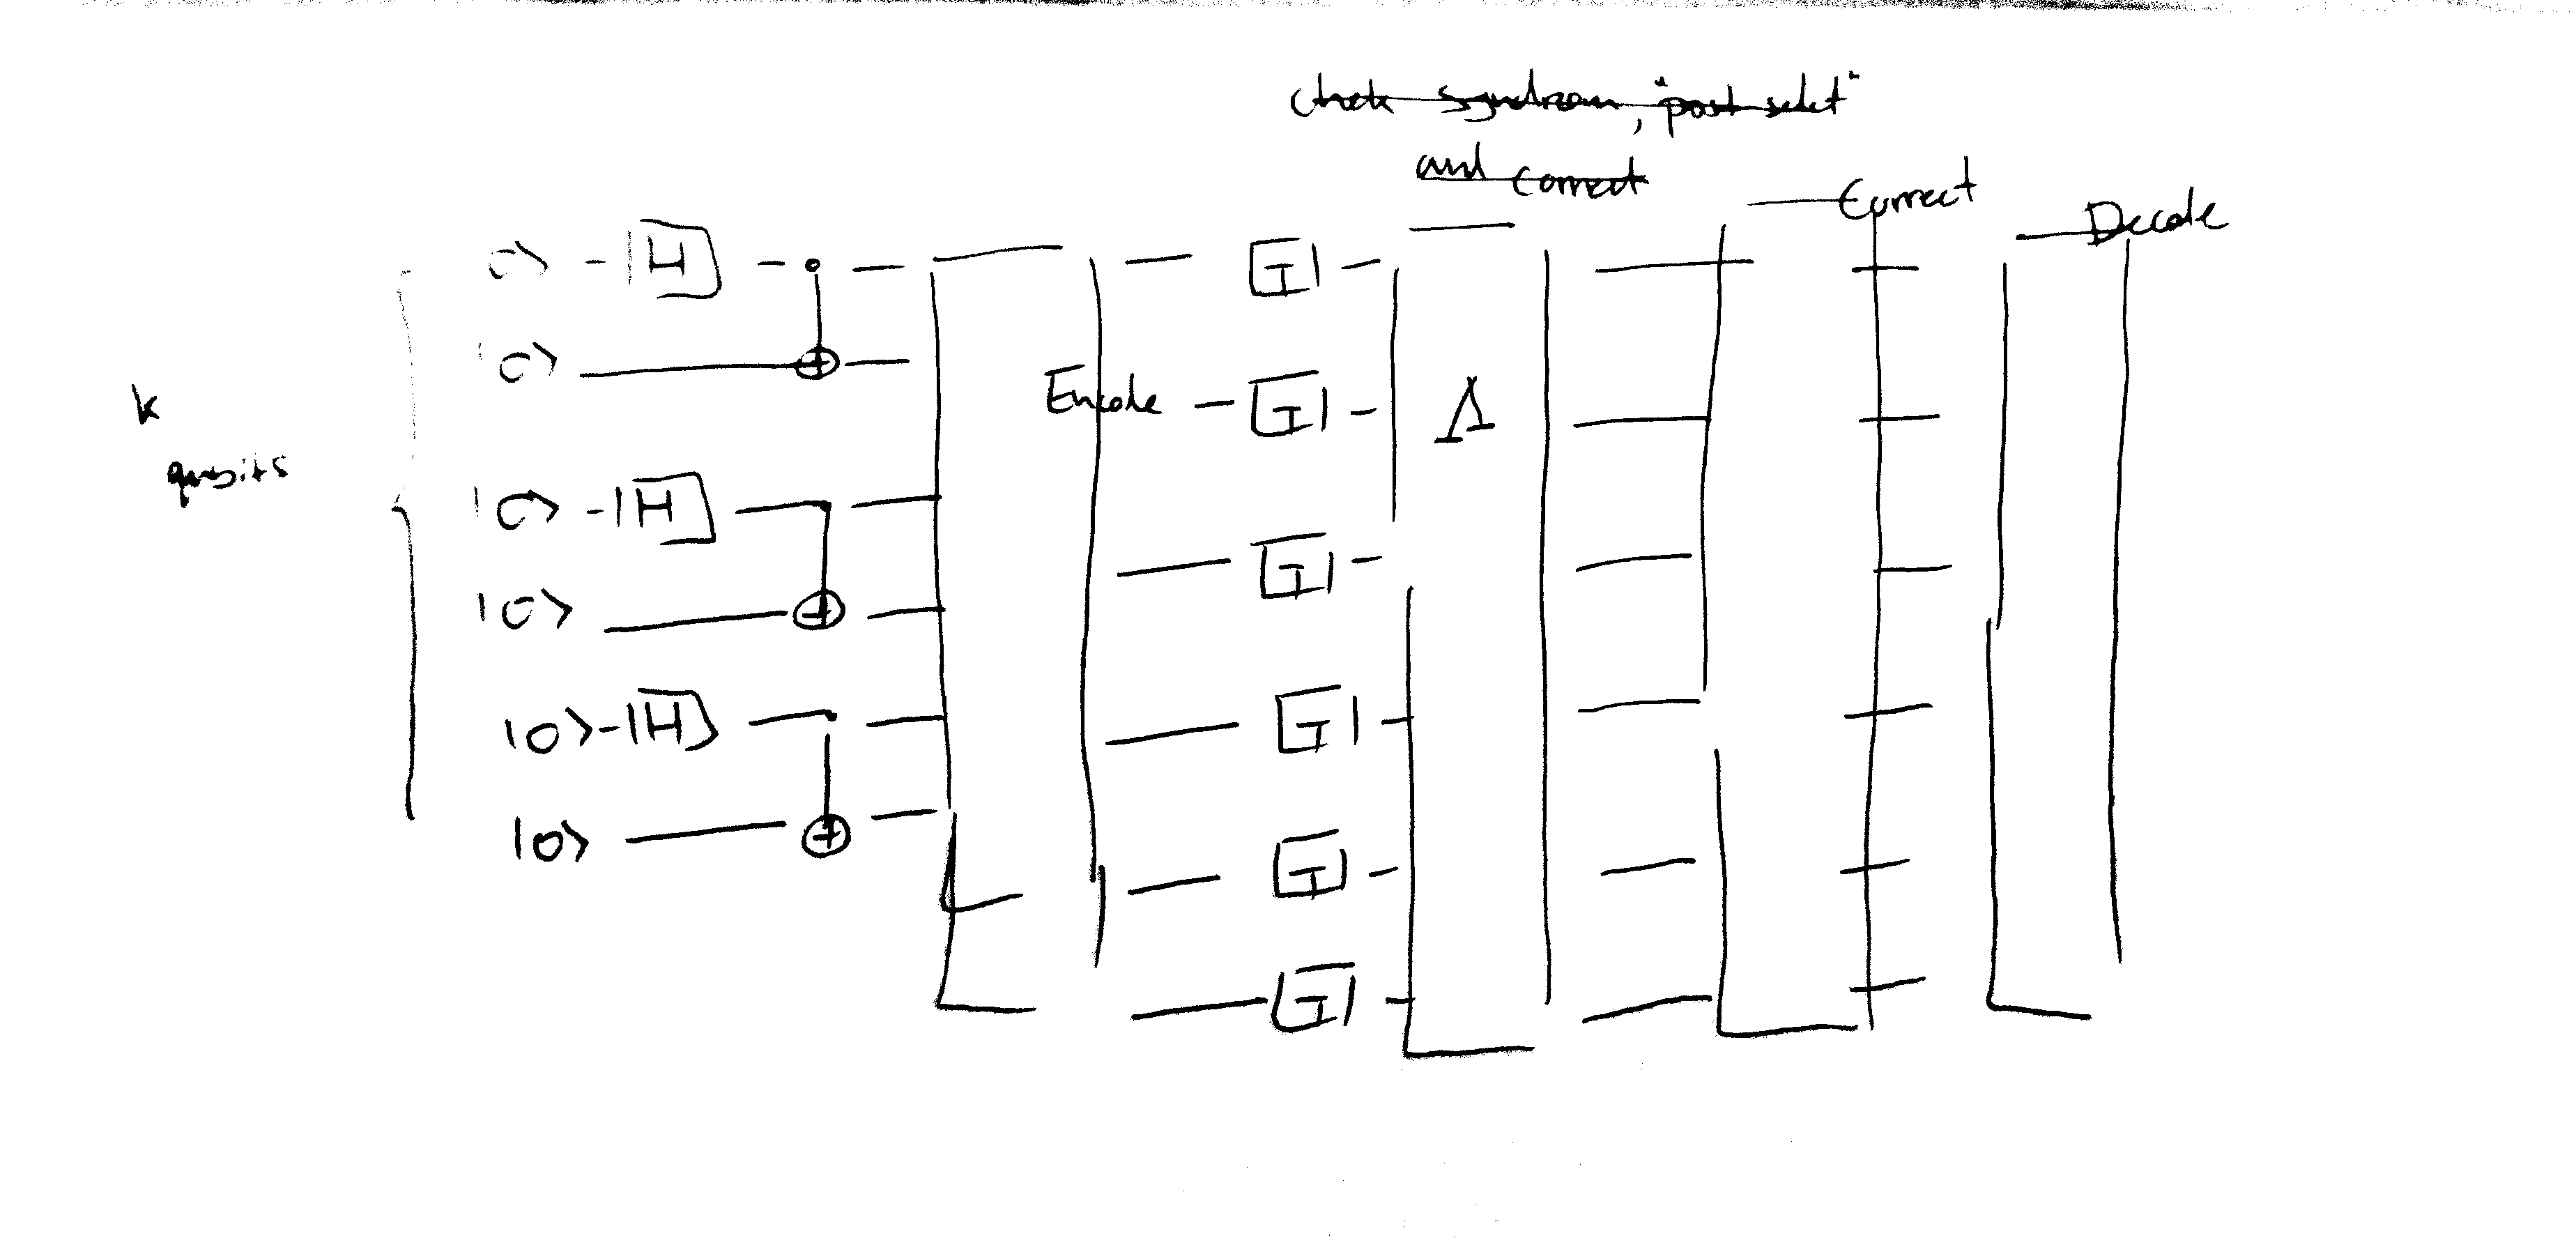
\includegraphics{distil.jpg-out.png}
}
  \caption{Quantum Circuit for distillation.}
  \label{fig:circuit}
\end{figure}

\end{document}







